\section{Evaluation}
\label{sec:eval}

We demonstrate the viability of our proposed scheme using a real cloud environment, Google Cloud.
We implement an indexing service, a search service and a
client application as standard Java services. The search service was deployed
on Google App Engine configured as an F4 class instance with a 2.4 GHz CPU and 512
MB of RAM. We utilized Google Blobstore for hosting index files because
it allows us to store and retrieve the complete index file efficiently.
This is in contrast to Google Datastore whose
entities can hold only a few bytes of data. As a result, when index entries increase,
read/write operations on index entries in the Datastore become more costly.

We evaluate the results of our approach on a dataset of 150 documents. 
These documents range in size from 5 MB to 100 MB, containing from 5000 to
129,000 keywords. The keywords were chosen to be at least 8 characters in
length and Porter stemming~\cite{porter} was applied to those keywords.
The client was a Lenovo Thinkpad 430 with a 2.6 GHz Intel Core(TM) i5-332M
CPU and 8 GB of RAM.

\subsection{Indexing Performance}
Figure \ref{fig:Index-Generation-Time} shows execution time for the index creation
and encryption 
processes over different input dataset sizes 
using a 64-bit Pascal Paillier key and a 3 KB bloom filter. The graph shows that,
despite using sliding window bloom filters, 
both encryption and index creation sizes increase linearly with input dataset size.

\begin{figure}[h!]
  \centering
  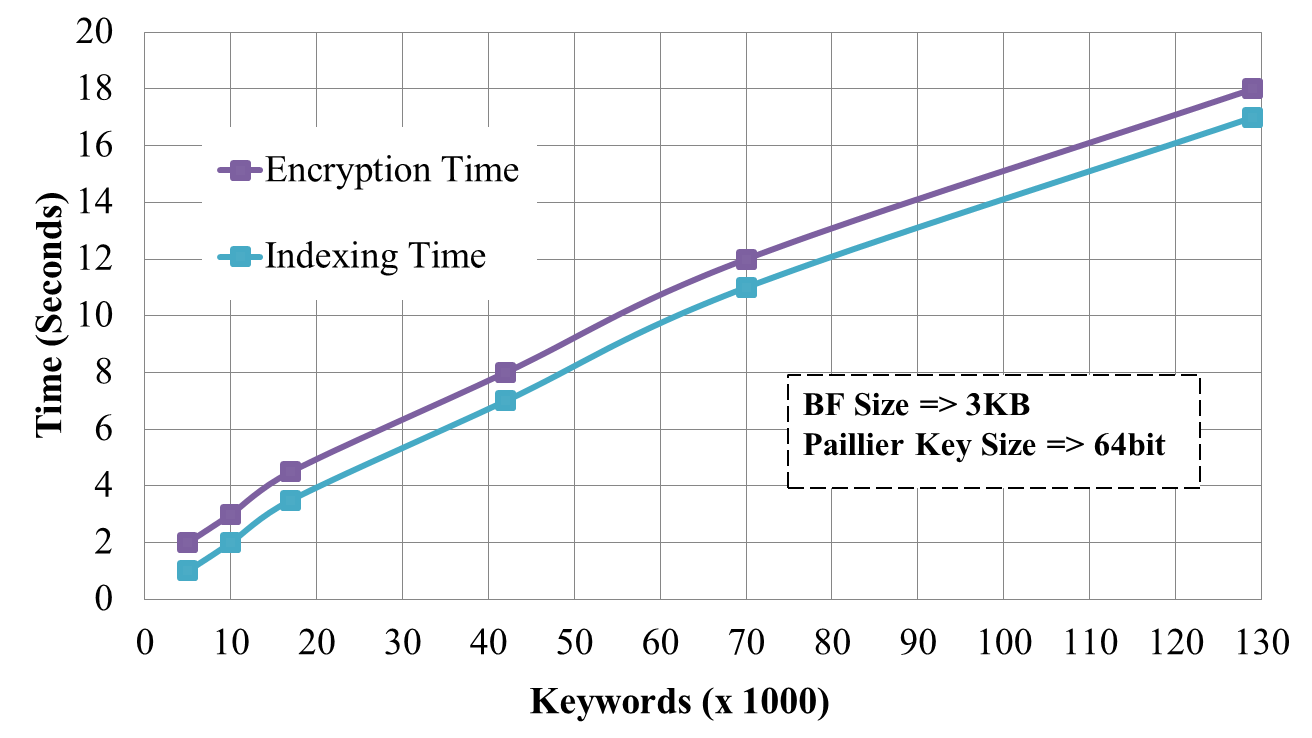
\includegraphics[width=3.5in]{figures/indexing_encryption_time.png}
  \caption{Index Generation Time}
  \label{fig:Index-Generation-Time}
\end{figure}

Paillier key size and bloom filter size both have a substantial impact on index file size. 
With the increase of bloom filter size, the false positive rate decreases but the size of each
index entry increases. The indexing time also increases, mainly because it takes longer
to upload a larger bloom filter to the cloud. 
A larger Paillier key size can help strengthen system security. However, with
increasing Paillier key size, index file size also increases proportionally and
out experiments shows that index size increases linearly with Paillier key size.

\subsection{Search Performance}

Search performance is evaluated in terms of data returned by a query, response
time, CPU cycles used to process a search request and the cost(\$) CSP will
charge for search queries. 
For private term matching and data returned, our implementation demonstrates
that by using our compression algorithm, data returned to the client
is 95\% less than traditional approaches and remains constant even when the size
of the bloom filter increases. This is shown in Figure \ref{fig:compress}.

\begin{figure}[h!]
  \centering
  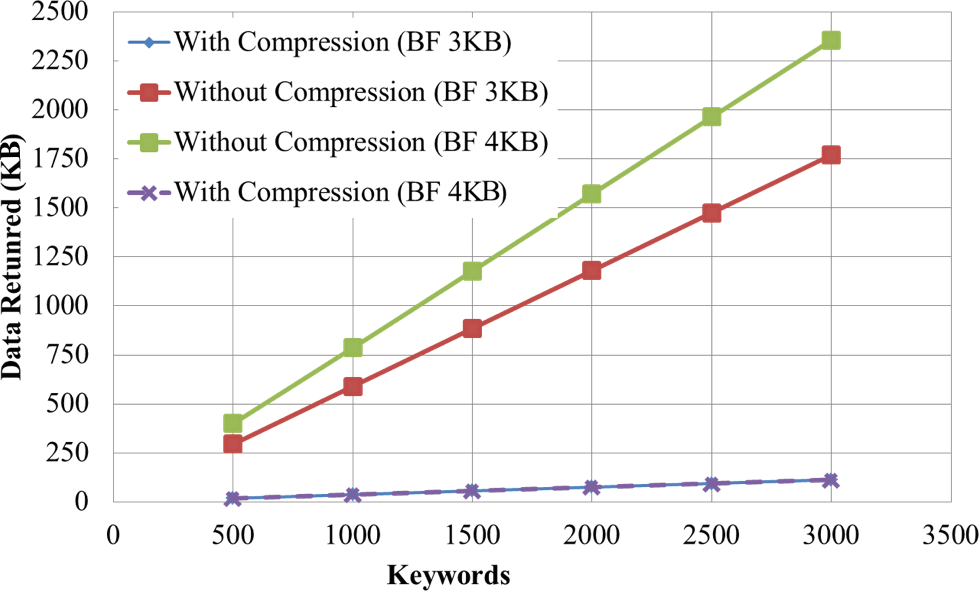
\includegraphics[width= 3.5in]{figures/comp_compare.png}
  \caption{Data returned by a search query: compressed vs uncompressed results}
  \label{fig:compress}
\end{figure}

We also measure the time it takes to extract the matching bloom filter values
from the compressed responses.
Table \ref{tab:search_response_time} show the results. As expected,
the extraction time increases linearly with the keyword count
on the server. The reason is that we add more keywords
keywords by adding more documents to the dataset and each document
has its own bloom filter index associated with it.

\begin{table}[th!]
\centering
\caption{Response time increases almost linearly with keyword count.}
\label{tab:search_response_time}
\begin{tabular}{| c | c | }
\hline
Keyword Count & Response Extraction Time (ms) \\
\hline
500  &  60 \\
1000 &  125 \\
1500 &  185 \\
2000 &  250 \\
2500 &  310 \\
3000 &  370 \\
\hline
\end{tabular}


\end{table}


\subsection{Cost Estimation and Response Times}

Finally, we evaluate the cost(\$) that CSP will charge to data owners for search
queries with partial matching. 
Our results, shown in Figure \ref{fig:cost_single_query}, demonstrate that a query
searching for a single keyword in a dataset having 500-3500 index entries will cost only \$0.000002 to \$0.00002 per 1000 similar
queries. Due to the sliding window bloom filter approach, 
all of the metrics increase only linearly ($O(n)$) with the number
of keywords on the server. This is substantially better than using a naive algorithm 
for partial matching, which would result in $O(nm)$ time complexity 
for $n$ keywords that are on average $m$ characters long. Crucially,
privacy is preserved throughout the search process because data is never
decrypted at the cloud or by any other untrusted system.

We obtained these cost metrics from Google App Engine logs for each data point. In
each log entry \emph{ms}, \emph{cpu\_ms} and \emph{cpm\_usd} depicts the wallclock response
time for a request, the \emph{normalized} CPU time needed to process the
request, and cost(\$) incurred for 1000 similar requests~\cite{google_cloud_logs}.


\begin{figure}
  \centering
  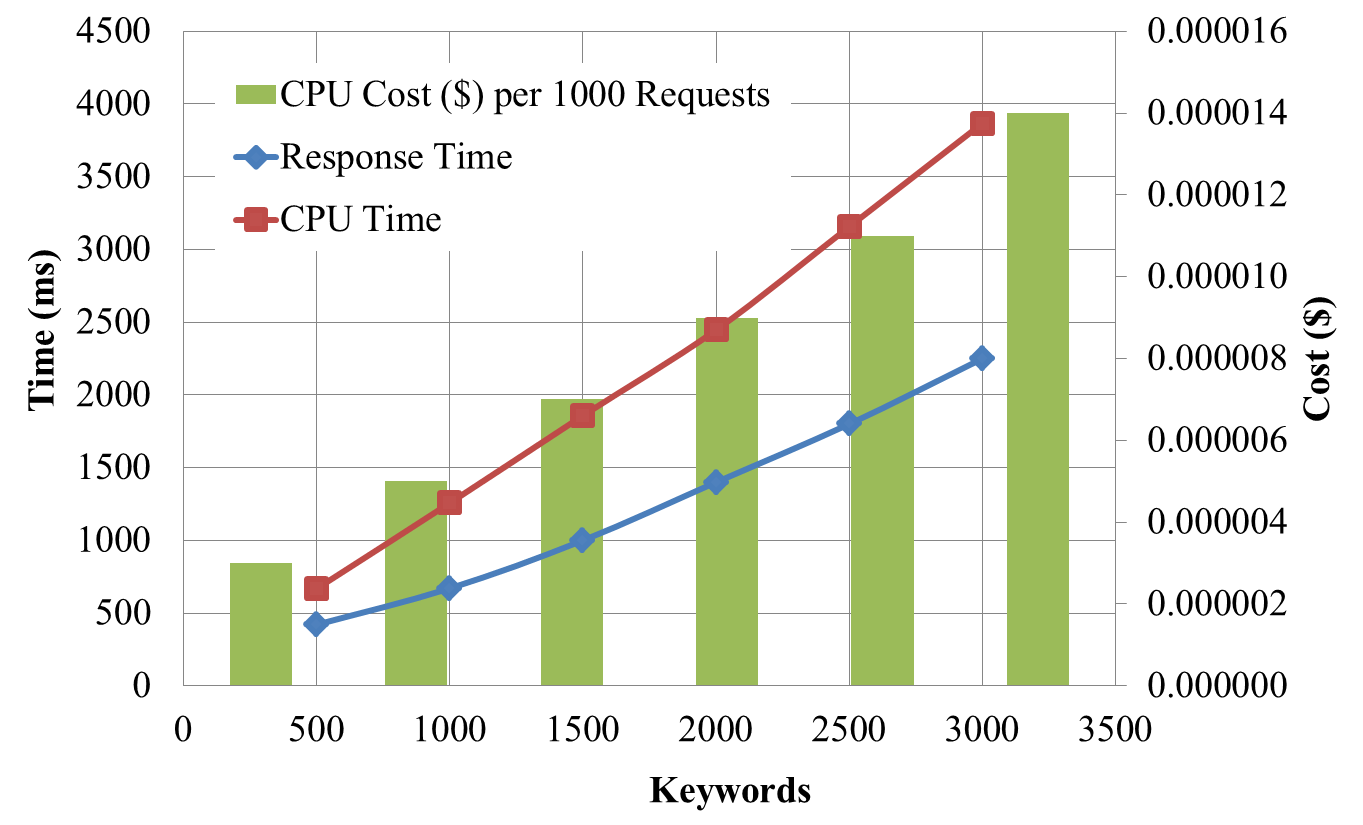
\includegraphics[width= 3.6in]{figures/cost_keywords_graph.png}
  \caption{Searching Cost(\$) with Single Keyword Query}
  \label{fig:cost_single_query}
\end{figure}
